\section{Methods}

\subsection{Design requirements from human physiology}

The jaw makes essential contributions to the chewing process such as generating the forces required to break down food, controlling the lower mandible motion
and giving sensory feedback. A robotic jaw should therefore be able to mimic these functions as closely as possible.
We first focus on force generation and range of motion, to build the structure of the chewing robot.
The design requirements are based on the human jaw anatomy and physiology, as summarized in Table~\ref{tab:functional_criteria}.


\begin{table}[H]
  \centering
  \begin{tabular}{@{}L{4.2cm}L{6.4cm}L{4.2cm}@{}}
    \toprule
    \textbf{Quantity} & \textbf{Values reported in the literature} & \textbf{Design requirement} \\
    \midrule
    DoF
      & 6-DoF: 3 translational (X, Y, Z) and 3 rotational (roll, pitch, yaw) \cite{6dof}
      & 6-DoF \\[2pt]
    \hline
    Vertical (compressive) bite force $F_{z}$ 
      & $600$ N chewing force in healthy adults \cite{chewing_force},\; $1243$ N maximum clenching force \cite{max_clenching_force}
      & $800$ N \\[2pt]
    
    \hline

    Lateral force $F_{x}$ 
      & $-72$ N (left) to $+53$ N (right) during maximal biting \cite{shear_force}
      & $\pm100$ N \\[2pt]
    \hline

    Anterior–posterior force $F_{y}$ 
      & $-10$ N (posterior) to $+30$ N (anterior) \cite{shear_force}
      & $\pm50$ N \\[2pt]
    \hline

    Mandibular motion range 
      & $14$ mm lateral shift, $11$ mm protrusion, $61$ mm mouth opening in healthy adults \cite{range_motion_required}
      & $\pm20$ mm (X, Y);\;\; $0$–$60$ mm (Z) \\[2pt]
  \bottomrule
  \end{tabular}
  \caption{Functional design requirements.}
  \label{tab:functional_criteria}
\end{table}


\subsection{Mechanical design}
\label{sec:mechanical_design}

This section details the key design decisions that led to the final mechanical design of the chewing robot and the resulting specifications.

\subsubsection{6-DoF mechanism}

The first major design decision was how to achieve 6-DoF for jaw motion. In the field of robotic mastication, two common approaches 
are used. The first is a biomechanically inspired design using linear actuators \cite{ChewingRobotLinearActuator} or combinations of actuated cables and 
springs \cite{ChewingRobotGums} to replicate muscle behavior. The second is a Stewart platform \cite{BristolChewingRobot}—a widely used 6-DoF parallel mechanism, often seen in 
motion simulators. See Figure~\ref{fig:stewart_platforms} for a visualization of the two approaches.

For this project, we chose the Stewart platform approach. Its well-defined kinematics and ease of control make it particularly suitable for our goal of 
replicating recorded human chewing motion. Because our control strategy is based on reproducing real motion trajectories, having a platform with 
straightforward inverse kinematics is a key advantage.

Stewart platforms generally come in two configurations: one based on rotary servo motors and one based on linear actuators, see Figure~\ref{fig:stewart_platforms}. 
We selected the linear actuator design for several reasons. It offers more efficient force transmission, a simpler kinematic model, and greater structural 
rigidity—all important factors when attempting to reproduce the forces involved in human chewing.

% 3 pictures side by side of the two approaches
\begin{figure}[H]
\centering
\begin{minipage}{.3\textwidth}
  \centering
  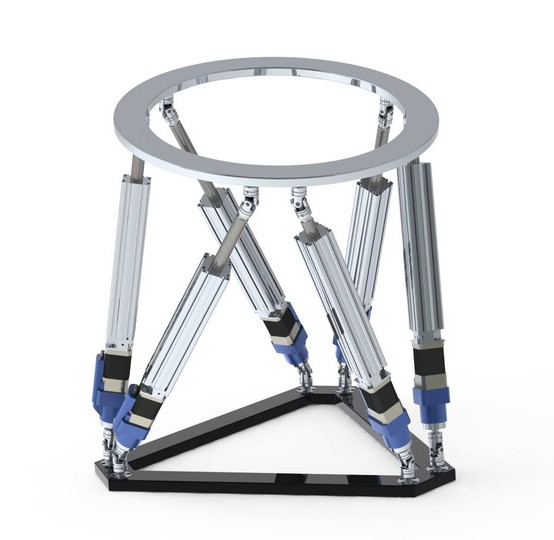
\includegraphics[height=4.6cm]{figures/linear_stewart_platform_2.jpg}
  \subcaption{}
  \label{fig:linear_stewart_platform}
\end{minipage}
\begin{minipage}{.3\textwidth}
  \centering
  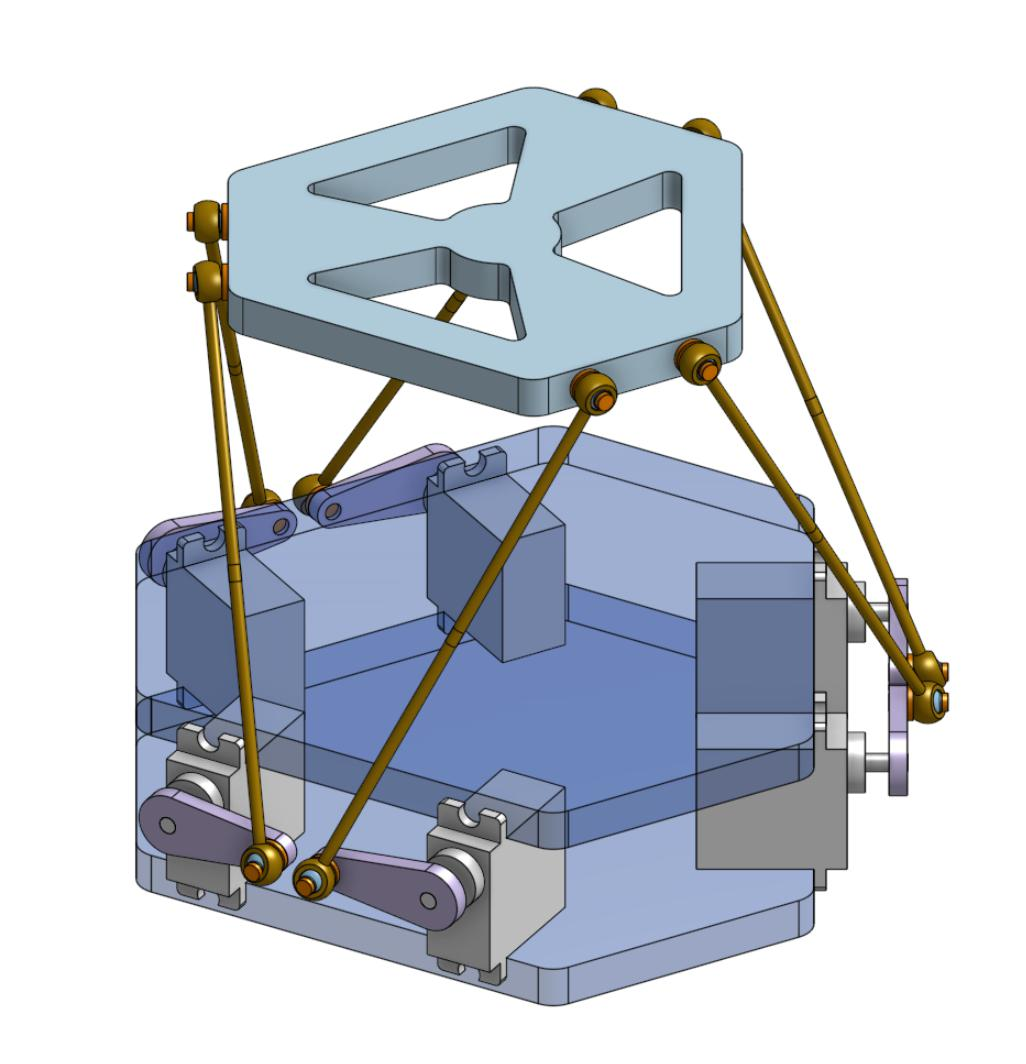
\includegraphics[height=4.6cm]{figures/rotary-stewart-plateform.jpg}
  \subcaption{}
  \label{fig:rotary_stewart_platform}
\end{minipage}
\begin{minipage}{.3\textwidth}
  \centering
  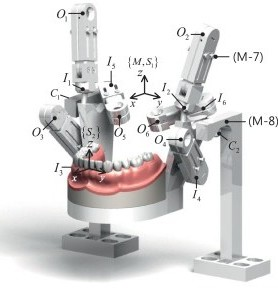
\includegraphics[height=4.6cm]{figures/6dof_jaw_cad.jpg}
  \subcaption{}
  \label{fig:biomechanically_inspired_design}
\end{minipage}
\caption{(a) Linear actuator-based Stewart platform. (b) Rotary servo motor-based Stewart platform. (c) Biomechanically inspired robotic jaw design\cite{ChewingRobotLinearActuator}.}
\label{fig:stewart_platforms}
\end{figure}

\subsubsection{Actuator requirements and selection}

The combination of high bite-force replication and position feedback demands actuators large enough to deliver both power and sensing hardware; their size 
therefore becomes a critical design constraint. Their stroke and force requirements are fixed by the functional criteria in Table \ref{tab:functional_criteria}. 

\paragraph{Design assumptions.}To compute the required actuator specifications, we assumed a minimum actuator mounting angle of at least 45° to the horizontal and the general 
geometry of the platform and base shown in Figure~\ref{fig:assumptions}. 
\begin{figure}[H]
\centering
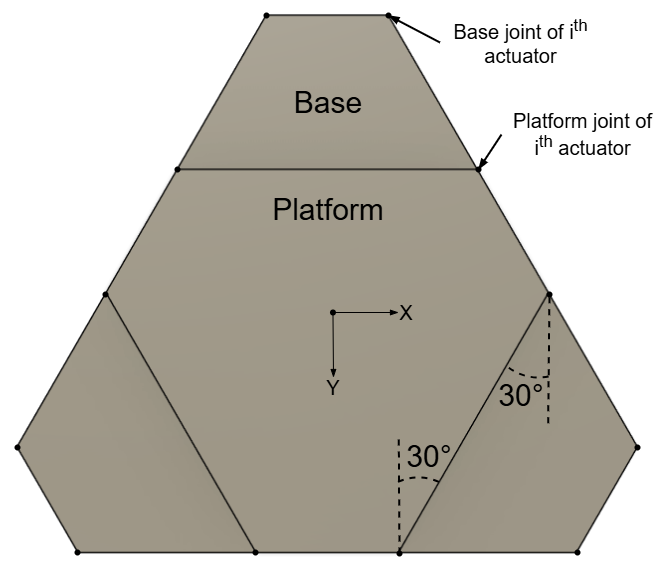
\includegraphics[width=0.5\textwidth]{figures/stewart_platform_assumption.drawio.png}
\caption{Top view of the base and platform design assumption.}
\label{fig:assumptions}
\end{figure}
\paragraph{Stroke length.}Guided by the workspace analysis from Masory et al. \cite{StewartPlatformWorkspace}, we prioritize achieving the necessary vertical range of motion, knowing that sufficient 
horizontal range would follow. The minimum required stroke length is:
\begin{equation}
l_{\text{min}} = \frac{z_{\text{max}} - z_{\text{min}}}{\sin(45^\circ)} = \frac{70\,\text{mm}}{\sin(45^\circ)} \approx 99\,\text{mm}
\end{equation}
\paragraph{Load.} To meet the minimum vertical force requirement of 800 N, each actuator must provide a load of at least:
\begin{equation}
F_{\text{min}} = \frac{F_{z,\text{min}}}{6 \cdot \sin(45^\circ)} = \frac{800\,\text{N}}{6 \cdot \sin(45^\circ)} \approx 189\,\text{N}
\end{equation}

With this minimum actuator force, we estimate the lateral (shear) and front-back force capacities as:
\begin{equation}
F_{x} \approx 2 \cdot \cos(45^\circ) \cdot F_{\text{min}} + 4 \cdot \cos(45^\circ) \cdot \sin(30^\circ) \cdot F_{\text{min}} \approx 534\,\text{N} \gg 100\,\text{N}
\end{equation}
\begin{equation}
F_{y} \approx 4 \cdot \cos(45^\circ) \cdot \cos(30^\circ) \cdot F_{\text{min}} \approx 462\,\text{N} \gg 50\,\text{N}
\end{equation}

These calculations show that ensuring the vertical force requirement is met also guarantees that shear forces in the x and y directions will exceed 
their respective targets.
\paragraph{Speed and feedback.}Since speed is not a requirement for this prototype, we prioritized force over velocity when selecting actuators. Position feedback is necessary 
for closed-loop control, as we use inverse kinematics to compute actuators lengths based on the desired platform pose.
\paragraph{Selection.}We selected the PA-14P-4-50 linear actuator, which meets both stroke and force requirements as seen in Table~\ref{tab:actuator_spec}. The dimensions 
of both base and platform, see Figure~\ref{fig:stewart_platform}, were chosen to accommodate the size of the actuators. The resulting vertical workspace 
of the platform is 118 mm, which is more than enough to cover the required 70 mm.

At mid-stroke, the actuators are positioned at an angle of 60° relative to the horizontal plane. Under this configuration, the theoretical maximum force 
outputs are: $F_{z,max} = 1155$ N (vertical), $F_{x,max} = 444$ N (lateral), and $F_{y,max} = 385$ N (anterior-posterior). 
All values surpass the design requirements specified in Table~\ref{tab:functional_criteria}. These are idealized values and do not account 
for frictional losses or mechanical inefficiencies.

\begin{figure}[H]
\centering
\begin{minipage}{.4\textwidth}
  \begin{table}[H]
    \centering
    \begin{tabular}{@{}p{3cm} p{2.5cm}@{}}
    \toprule
    \textbf{Parameter} & \textbf{Value}\\
    \midrule
    Stroke length & 101 mm \\
    Max force & 222.4 N \\
    Speed (no load) & 28 mm/s \\
    Speed (full load) & 21 mm/s \\
    Position feedback & Potentiometer \\
    Protection class & IP54 \\
    Power supply & 12 V DC \\
    \bottomrule
    \end{tabular}
    \caption{PA-14P-4-50 specifications.}
    \label{tab:actuator_spec}
  \end{table}
\end{minipage}
\begin{minipage}{.5\textwidth}
  \centering
  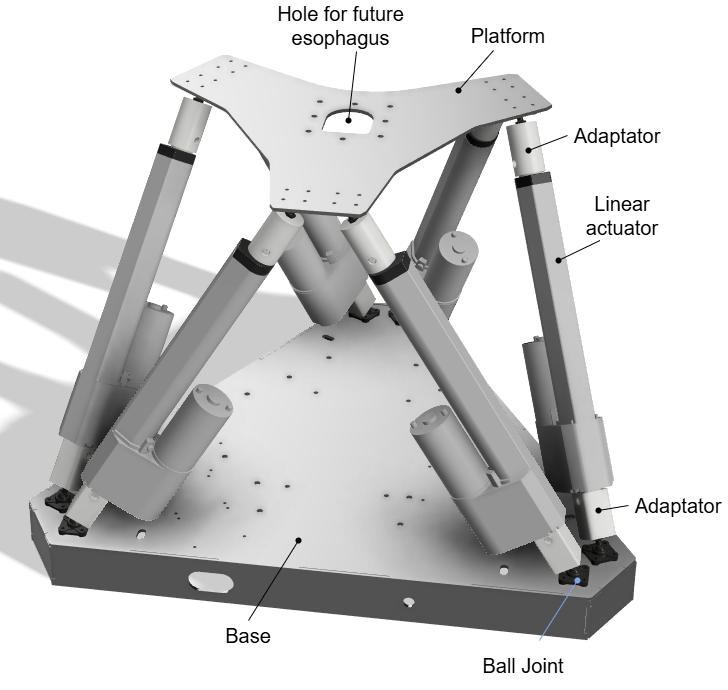
\includegraphics[width=\textwidth]{figures/stewart_platform_annotated.drawio.png}
  \caption{Final Stewart platform design.}
  \label{fig:stewart_platform}
\end{minipage}
\end{figure}

\subsubsection{Jaw subassemblies}

Next, we designed the lower and upper jaws, which are attached to the platform and base respectively. 
\paragraph{Lower jaw.}The lower jaw, Figure~\ref{fig:lower_jaw}, is mounted on the moving platform and elevated using four aluminum rods. This elevation 
provides two main advantages: it creates a clear line of sight to place a motion capture marker on the gnathion, and it 
leaves space beneath the jaw for integrating a future esophagus module. The mandibular teeth are fixed to a rigid plate 
and positioned slightly forward to leave room for a future tongue module. This plate already accommodates a hole for a future esophagus module.
\paragraph{Upper jaw.}The upper jaw, Figure~\ref{fig:upper_jaw}, is mounted on a rigid frame made of aluminum rods to ensure sufficient stability and stiffness under loading. This 
rigidity is essential to resist the forces applied by the lower jaw during chewing. Three-axis load cells are installed on the 
upper jaw mounting plate to measure both vertical and lateral forces during contact. Two acrylic adaptor plates connect these load 
cells to the maxillary teeth. The top adaptor has a central opening reserved for a future camera, which will be used to observe food 
behavior during mastication.
\paragraph{Exchangeable teeth.}Both the maxillary and mandibular teeth are designed to be easily replaceable through the use of acrylic adaptor plates. This modularity 
allows for testing different tooth shapes, materials, and conditions (e.g., healthy, aged, or damaged teeth), which will be important for 
future studies on chewing development and masticatory disorders.

\begin{figure}[H]
\centering
\begin{minipage}{.5\textwidth}
  \centering
  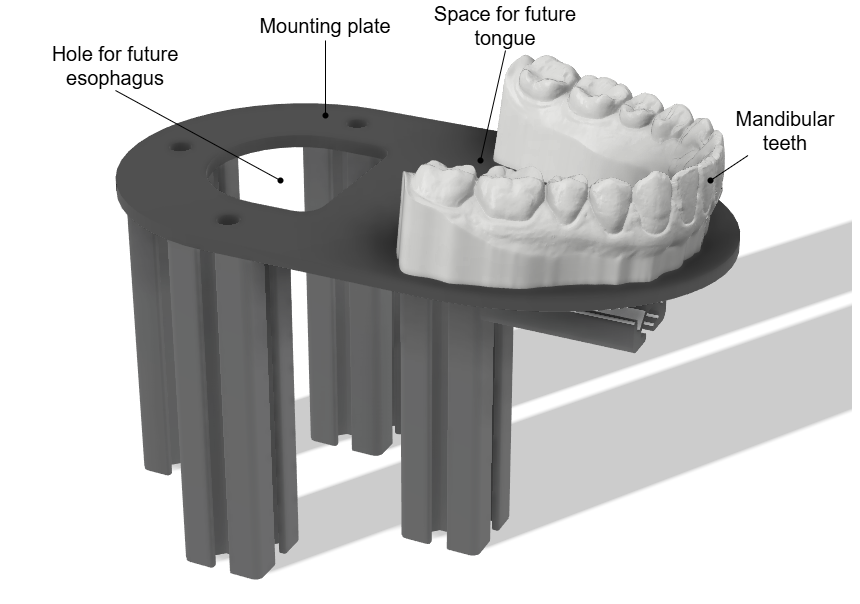
\includegraphics[width=\textwidth]{figures/lower_jaw_annotated.drawio.png}
  \subcaption{}
  \label{fig:lower_jaw}
\end{minipage}
\begin{minipage}{.4\textwidth}
  \centering
  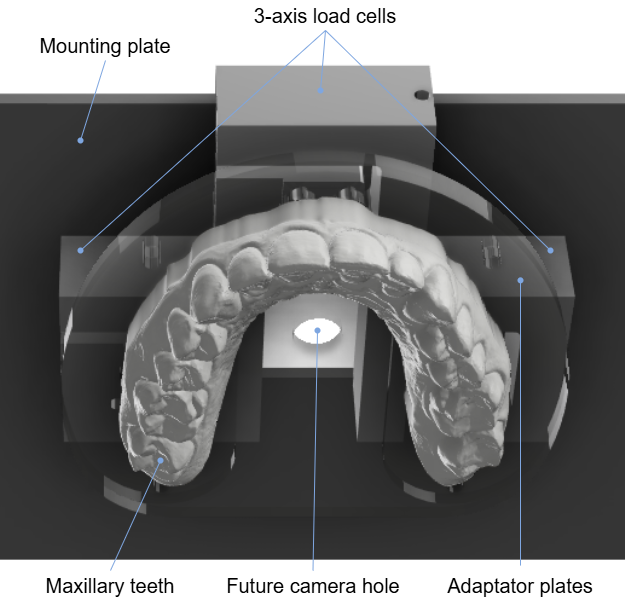
\includegraphics[width=\textwidth]{figures/upper_jaw_annotated.drawio.png}
  \subcaption{}
  \label{fig:upper_jaw}
\end{minipage}
\caption{(a) Annotated lower jaw design. (b) Annotated upper jaw design. }
\label{fig:jaws}
\end{figure}

\subsubsection{Full assembly}

\paragraph{Final workspace.}The final design is shown in Figure~\ref{fig:overview}. Pictures of the built robot are included in Section~\ref{sec:real_pictures} of the Appendix. The height of the upper jaw subsystem was set slightly below the platform's maximum 
vertical reach—roughly centered in the middle of its vertical workspace. This positioning ensures that the robot can apply maximum vertical 
force when the mandibular and maxillary teeth are in contact, while still allowing enough range to meet angular requirements during chewing. 
A detailed view of the vertical workspace can be found in Figure~\ref{fig:vertical_workspace}. The lateral and anterior-posterior workspaces are 
constrained by the upper jaw frame and are approximately $\pm$60 mm and $\pm$80 mm, respectively. 
The base is designed as a hollow box to house the electronics 
described in Section~\ref{sec:control}. 

\begin{figure}[H]
\centering
\begin{minipage}{.4\textwidth}
  \centering
  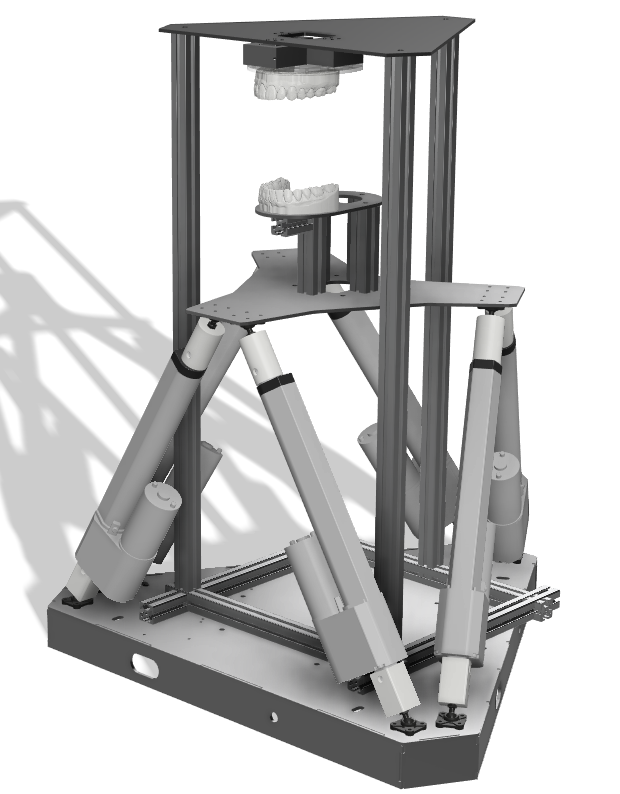
\includegraphics[width=\linewidth]{figures/overview.png}
  \subcaption{}
  \label{fig:overview}
\end{minipage}
\begin{minipage}{.4\textwidth}
  \centering
  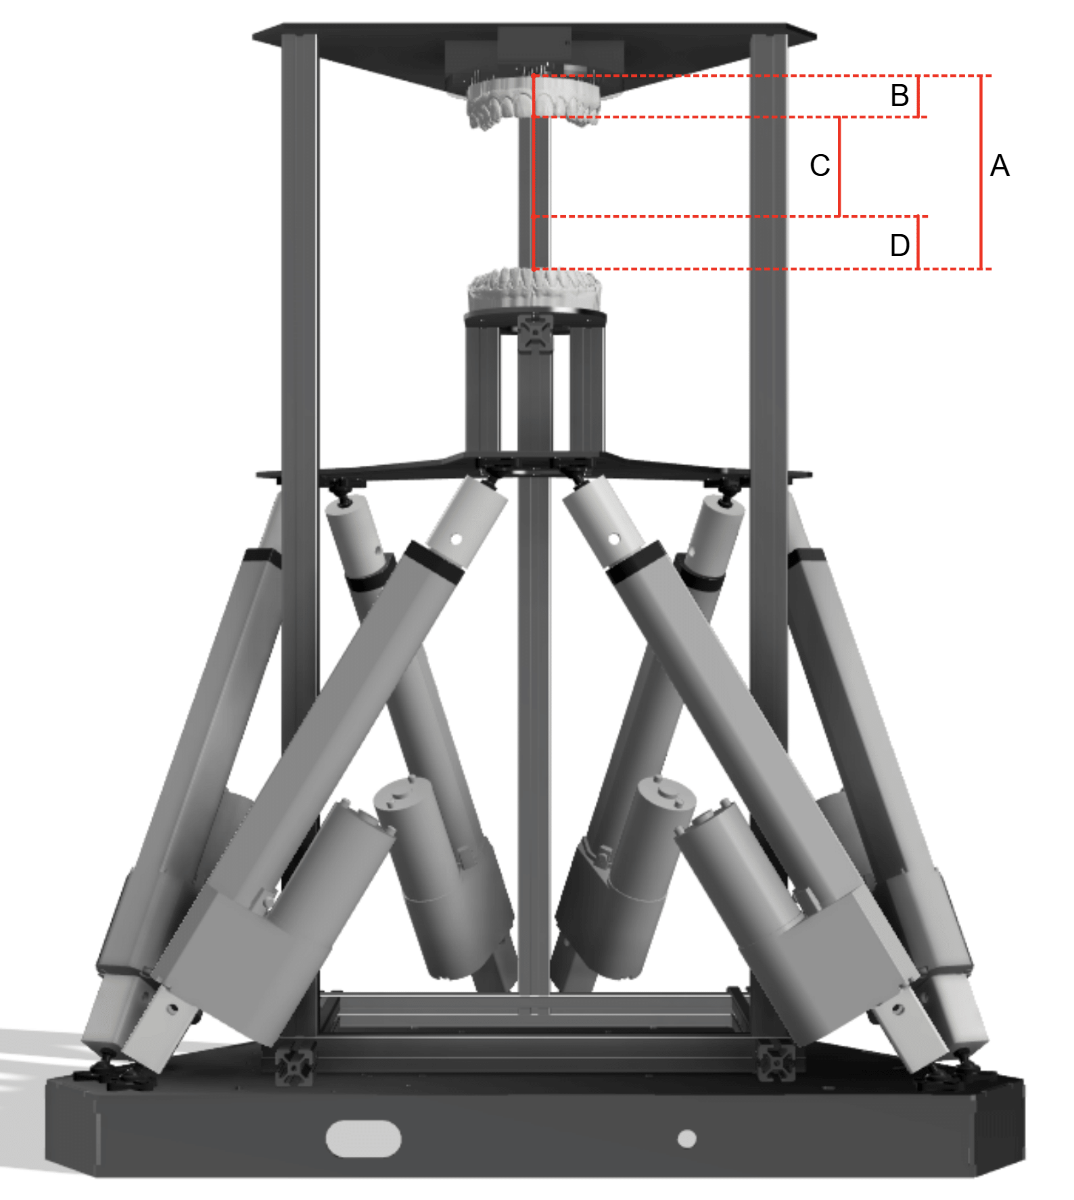
\includegraphics[width=\linewidth]{figures/workspace_2.drawio.png}
  \subcaption{}
  \label{fig:vertical_workspace}
\end{minipage}
\caption{(a) Final design overview. (b) Workspace design: A-Full vertical workspace of 118 mm; B-Upper margin of 25 mm; C-Working chewing volume of 60 mm; D-Bottom margin of 33 mm.}
\label{fig:mecha_design}
\end{figure}

\paragraph{Material selection.}The base, platform, lower jaw mount, and upper jaw mount are all made out of steel, see Table~\ref{tab:mecha_materials}. 
Although heavier than aluminum, steel offers significantly higher stiffness, with a Young's modulus of 190-210 GPa. This makes it a better choice 
for components that require high rigidity and minimal deformation under load. Additionally, steel's weldability makes it practical for future 
modifications—for example, adding reinforcement ribs to the upper jaw mounting plate to further improve structural stability.

\begin{table}[H]
\centering
\begin{tabular}{@{}p{3.5cm} p{4.6cm} p{3cm}@{}}
\toprule
\textbf{Subassembly} & \textbf{Part} & \textbf{Material} \\
\midrule
\multirow{3}{*}{Stewart Platform} 
    & Base & Steel \\
    & Platform & Steel \\
    & Adapter & PLA \\
\midrule
\multirow{2}{*}{Lower Jaw} 
    & Lower jaw mounting plate & Steel \\
    & Mandibular teeth & PLA \\
\midrule
\multirow{3}{*}{Upper Jaw} 
    & Upper jaw mounting plate & Steel \\
    & Upper jaw adapter plates & Acrylic \\
    & Maxillary teeth & PLA \\
\bottomrule
\end{tabular}
\caption{Mechanical design materials.}
\label{tab:mecha_materials}
\end{table}

\paragraph{Waterproofing.}
As the robot is designed to eventually include a saliva module, it is important to ensure that the electronics and mechanical components are protected from moisture.
First, we protected the steel parts with a layer of paint to prevent rusting. Then on both the upper and bottom side of the base, a plastic sheet was added 
to isolate the electronics from the steel base and prevent water from entering inside the box and damaging the electronics. 
Finally, the linear actuators are IP54-rated, meaning they are protected against dust and splashes of water from any direction, see Table~\ref{tab:actuator_spec}.

\paragraph{Specifications summary.}The final specifications of the chewing robot are summarized in Table~\ref{tab:final_specs}. It is worth noting that 
the center of mass height is expected to decrease further once the electronic components are installed within the base enclosure.

\begin{table}[H]
\centering
\begin{tabular}{ l l }
\toprule
\textbf{Parameter} & \textbf{Value} \\
\midrule
Total mass & 21 kg \\
Dimensions (L x W x H) & 530 mm x 460 mm x 600 mm \\
Center of mass & 150 mm above base center \\
Vertical force capacity ($F_{z,\mathrm{max}}$) & 1155 N \\
Lateral force capacity ($F_{x,\mathrm{max}}$) & 444 N \\
Anterior-posterior force capacity ($F_{y,\mathrm{max}}$) & 385 N \\
Vertical workspace & 118 mm \\
Lateral workspace & $\pm$ 60 mm \\
Anterior-posterior workspace & $\pm$ 80 mm \\
Working vertical chewing volume & 60 mm \\
Actuator stroke length & 101 mm \\
Max actuator speed (no load) & 28 mm/s \\
Max actuator speed (full load) & 21 mm/s \\
Moisture protection & Painted + plastic sheets + IP54-rated actuators \\
\bottomrule
\end{tabular}
\caption{Final specifications of the chewing robot.}
\label{tab:final_specs}
\end{table}

\subsection{Control system}
\label{sec:control}

This section describes the hardware and software architecture of the chewing robot as well as the control strategy.

\subsubsection{Hardware (electronics)}
A Teensy~4.1 (600 MHz ARM Cortex-M7, single-precision FPU) executes the control loop. % at \SI{100}{\hertz}. %? %todo: add ref for the freq/reason
Its key peripherals are:  
\begin{itemize}[nosep]
    \item three \SI{12}{\ampere} dual DC motor drivers (DF Robot) controlling the six linear actuators;
    \item two multiplexers connected to :
    \begin{itemize}
      \item six analogue inputs reading potentiometer position feedback from the linear actuators;
      \item three transmitters for the load cells mounted on top of the maxilla;
    \end{itemize}
    \item an on-board micro-SD slot used for trajectory files and calibration data.
\end{itemize}
As for the power supply, the Teensy is powered by a \SI{5}{\volt} USB connection from the host computer, which also provides the communication link. 
The \SI{3.3}{\volt} from the Teensy gives the logic levels for the motor drivers and load-cell transmitters. 
A \SI{12}{\volt} AC/DC power supply powers the motor drivers directly, which in turn power the linear actuators. A \SI{24}{\volt} AC/DC power supply is used to power the load-cell transmitters. 
The full electronics schematic is shown in Fig.~\ref{fig:elec_schematic}. More details on the electronics connections to the Teensy~4.1 are shown in Fig.~\ref{fig:connections_teensy} in the Appendix.

\begin{figure}[H]
\centering
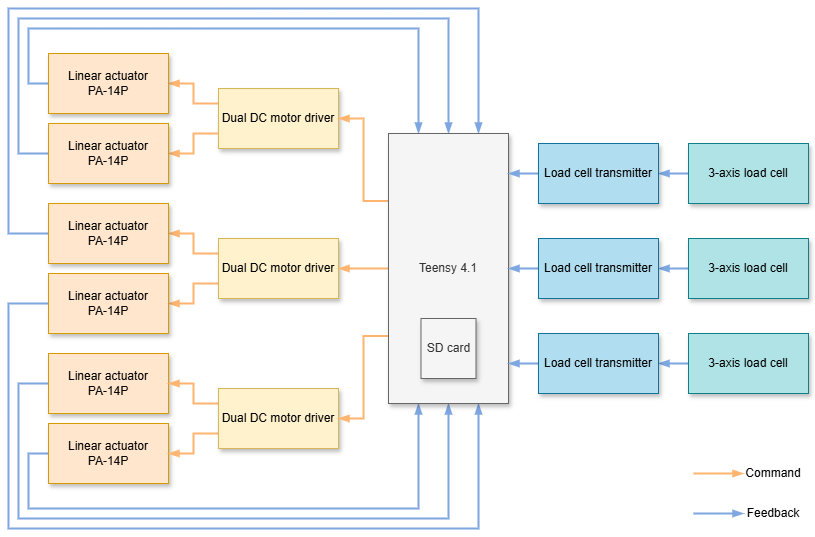
\includegraphics[width=\textwidth]{figures/elec_schematic.drawio.png}
\caption{Electronics schematic.}
\label{fig:elec_schematic}
\end{figure}

\subsubsection{Software architecture}
The main code \cite{githu_repo} was developed in object-oriented C++ using the Arduino framework and runs on the Teensy~4.1. 
The central class \texttt{RobotController} maintains the finite-state machine in Fig.~\ref{fig:state_machine} and manages two
 modules:  
\begin{itemize}[nosep]
    \item \texttt{StewartPlatform}: inverse kinematics, trajectory interpolation, and low-level actuator commands;
    \item \texttt{ForceSensing}: continuous load-cell acquisition and filtering;
\end{itemize}

\begin{figure}[H]
\centering
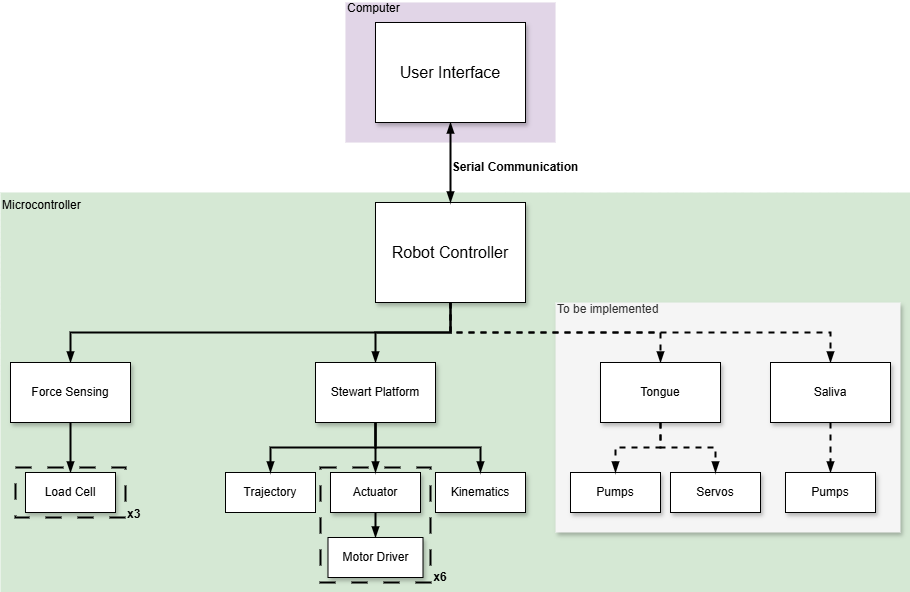
\includegraphics[width=0.9\textwidth]{figures/code_structure.drawio.png}
\caption{Overall code structure.}
\label{fig:code_structure}
\end{figure}
The controller is designed to be modular, allowing for easy addition of new modules such as a tongue or saliva module in the future. 

The three controller states are:
\begin{enumerate}
    \item \textbf{Stop} – return to home pose; reload trajectory if the user selects a new file;
    \item \textbf{Calibrate} – user can manually change the initial $(x,y,z)$ position via the GUI;
    \item \textbf{Move} – replay the selected trajectory.
\end{enumerate}

\begin{figure}[H]
\centering
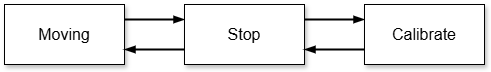
\includegraphics[width=0.6\textwidth]{figures/state_machine.drawio.png}
\caption{Robot controller state machine.}
\label{fig:state_machine}
\end{figure}

The host PC runs a lightweight python GUI built with PyQt5, which is used to send high-level commands, such as initiating state transitions. It also collects sensory feedback 
through the serial terminal. Upon pressing the Stop button, the interface generates plots from the recorded data. The GUI layout is shown in Figure~\ref{fig:gui}.

\begin{figure}[H]
  \centering
  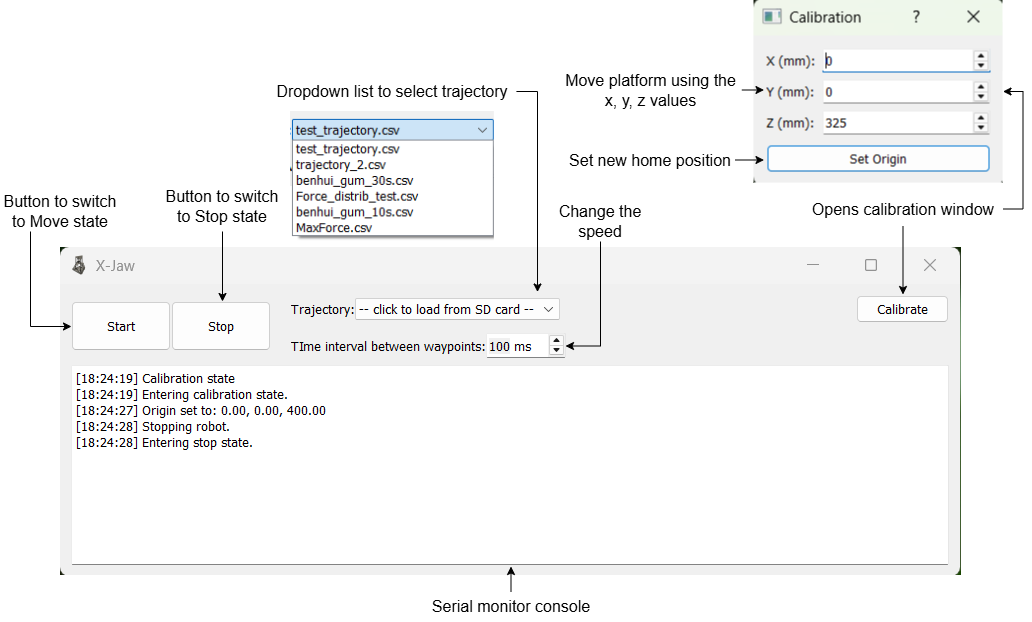
\includegraphics[width=\textwidth]{figures/gui.drawio.png}
  \caption{Robot controller GUI.}
  \label{fig:gui}  
\end{figure}

\subsubsection{Stewart platform control}

The Stewart platform is controlled by the \texttt{StewartPlatform} class, which manages the trajectory, platform kinematics, and high-level actuator control. 
Its real-time loop executes every \SI{10}{\milli\second} (\SI{100}{\hertz}). 
The platform follows a 3D trajectory (x, y, z, roll, pitch, yaw) from a .csv file on the micro-SD card. 
See section \ref{sec:motion-capture} for details on the recording protocol and data processing. 
Each pose is defined by its position ${\bf t}=(x,y,z)$ and orientation given by the Euler angles $(\phi,\theta,\psi)$,
 which are the roll, pitch, and yaw angles respectively. 
The trajectory is then interpolated using a Catmull-Rom spline with a fixed time step chosen by the user.

\paragraph{Inverse kinematics}
For each pose in the trajectory, \texttt{Kinematics} computes the lengths of the six linear actuators that will achieve 
the desired pose of the platform, i.e. the inverse kinematics. First, let's define our system. The base is defined as the 
global reference frame with orthogonal axes (x, y, z), while the platform is associated with a local orthogonal coordinate 
system (x', y', z'). Figure~\ref{fig:robot_referential} shows a visualization of these axes. The platform has six degrees 
of freedom relative to the base: three translational and three rotational. To account for the platform's rotation, we use the 
standard rotation matrix $R(\phi,\theta,\psi)$, which is defined as the product of three rotation matrices about 
the $Z$, $Y$, and $X$ axes:
\[
R(\phi,\theta,\psi) = R_Z(\psi) R_Y(\theta) R_X(\phi) =
\begin{pmatrix}
\cos\psi & -\sin\psi & 0 \\
\sin\psi & \cos\psi & 0 \\
0 & 0 & 1
\end{pmatrix}
\begin{pmatrix}
\cos\theta & 0 & \sin\theta \\
0 & 1 & 0 \\
-\sin\theta & 0 & \cos\theta
\end{pmatrix}
\begin{pmatrix}
1 & 0 & 0 \\
0 & \cos\phi & -\sin\phi \\
0 & \sin\phi & \cos\phi
\end{pmatrix}
\]

In our case, the center of rotation is the gnathion, defined as a fixed point ${\bf c}$ and visualized in Figure~\ref{fig:lower_jaw}, rather than the origin of the platform. Therefore, 
the platform joints ${\bf p}_i$, $i$ being the actuator index, are first rotated about the gnathion and then translated by the user-defined 
home position ${\bf T}=(x,y,z)$, resulting in the global coordinates of the platform joints:
\[
{\bf q}_i = R\bigl({\bf p}_i-{\bf c}\bigr)+{\bf c}+{\bf T}.
\]

Figure~\ref{fig:kinematic_schematic} shows the kinematic schematic for the $i^{th}$ actuator.
Finally, the actuator length is the Euclidean distance to the fixed base joint ${\bf b}_i$:
\[
\ell_i = \lVert {\bf q}_i-{\bf b}_i\rVert_2.
\]

\begin{figure}[H]
\centering
\begin{minipage}{.45\textwidth}
  \centering
  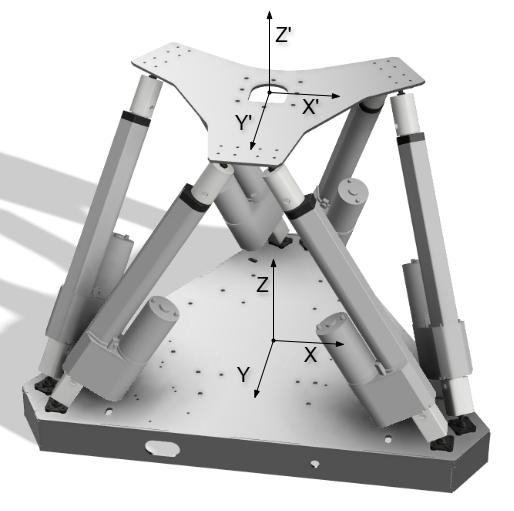
\includegraphics[height=6cm]{figures/robot_referential.drawio.png}
  \caption{Robot referential.}
  \label{fig:robot_referential}
\end{minipage}
\begin{minipage}{.5\textwidth}
  \centering
  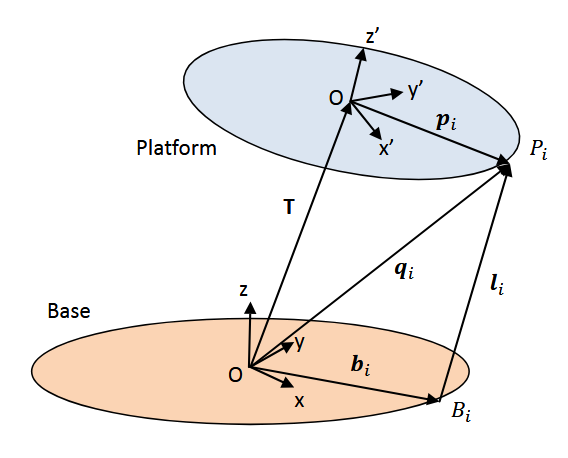
\includegraphics[height=6.3cm]{figures/kinematic_schematic.png}
  \caption{Schematic of the Stewart platform kinematics for the $i^{th}$ actuator \cite{instructables2024}.}
  \label{fig:kinematic_schematic}
\end{minipage}
\end{figure}

\paragraph{PI controller}
For each actuator, its desired length is sent to a PI position controller, see Figure~\ref{fig:actuator_pi}. The PI gain values 
are set to $K_P=25$ and $K_I=0.1$, which were determined empirically to achieve a good trade-off between responsiveness and stability. 
An anti-windup mechanism is implemented to prevent the integral term from growing too large, which could lead to overshooting. 
To minimize the noise of the potentiometer feedback, we apply a low-pass filter averaging the last 10 samples.
\begin{figure}[H]
\centering
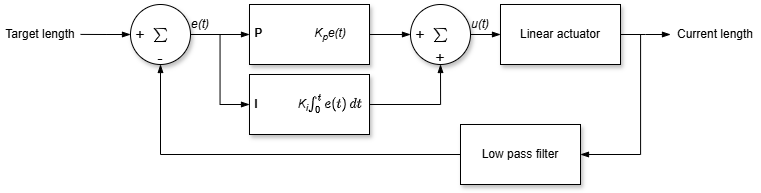
\includegraphics[width=\textwidth]{figures/actuator_pi.drawio.png}
\caption{Position PI controller for the linear actuators.}
\label{fig:actuator_pi}
\end{figure}

\subsubsection{Force sensing}
The \texttt{ForceSensing} module is responsible for acquiring and processing data from the three tri-axial load cells mounted on the upper jaw. 
Each load cell is represented by an instance of the \texttt{LoadCell} class, which performs signal conditioning on the raw sensor data. 
Specifically, a low-pass filter is applied by averaging the last 10 samples to reduce high-frequency noise.

According to the manufacturer's calibration data, the load cell output from the transmitter is sufficiently linear for direct mapping, see 
Figure~\ref{fig:load_cell_calibration}. Based on this, the \texttt{LoadCell} class linearly scales the filtered signal to a calibrated 
force range of [0, 500] N. To eliminate static bias introduced by preloading or assembly stress, each load cell is automatically tared at system startup.

\begin{figure}[H]
\centering
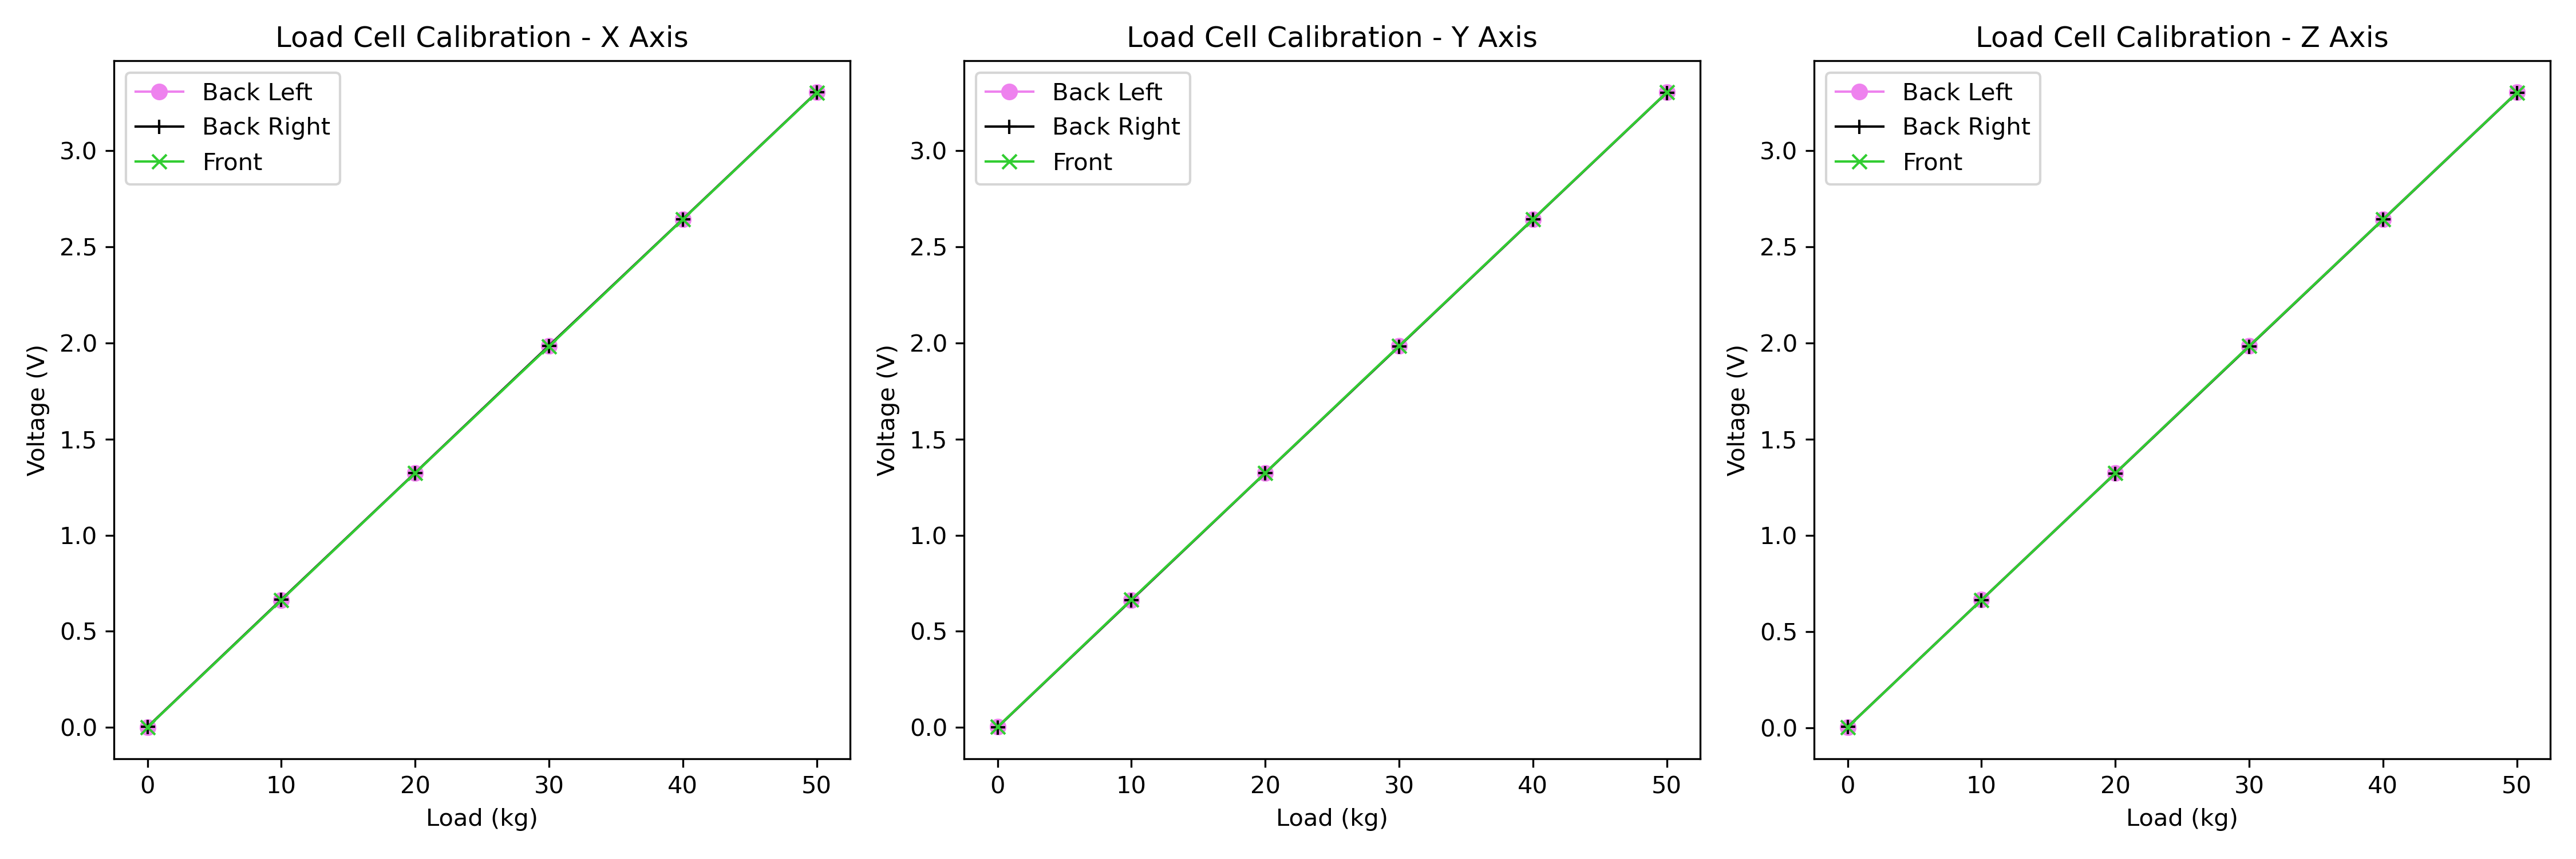
\includegraphics[width=\textwidth]{figures/load_cell_calibration.png}
\caption{Load cell calibration data.}
\label{fig:load_cell_calibration}
\end{figure}

The \texttt{ForceSensing} module aggregates the force data from all three load cells to compute the total force applied on the upper jaw. 
Since each load cell only measures force in the positive direction of its axis, their physical orientation must be accounted for during summation. 
This configuration is illustrated in Figure~\ref{fig:load_cells_axis}. The total forces in the x, y, and z directions are calculated as:
\begin{equation}
  F_{x,total} = F_{x,front} + F_{x,backL} - F_{x,backR},
\end{equation}
\begin{equation}
  F_{y,total} = F_{y,front} + F_{y,backL} - F_{y,backR},
\end{equation}
\begin{equation}
  F_{z,total} = F_{z,front} + F_{z,backL} + F_{z,backR}.
\end{equation}
% For now, the \texttt{ForceSensing} module primarily serves as a safety mechanism. If the total measured force exceeds predefined 
% thresholds—200 N in the z-direction, 60 N in x, or 50 N in y—the module fails and triggers \texttt{RobotController} to transition to \texttt{Stop} mode 
% to prevent damage to the robot.

\begin{minipage}{0.50\textwidth}
For now, the \texttt{ForceSensing} module primarily serves as a safety mechanism and force feedback recording. If the total measured force exceeds predefined 
thresholds—200 N in the z-direction, 60 N in x, or 50 N in y—the module fails and triggers \texttt{RobotController} to transition to \texttt{Stop} mode 
to prevent damage to the robot.
\end{minipage}
\hfill
\begin{minipage}{0.40\textwidth}
  \centering
  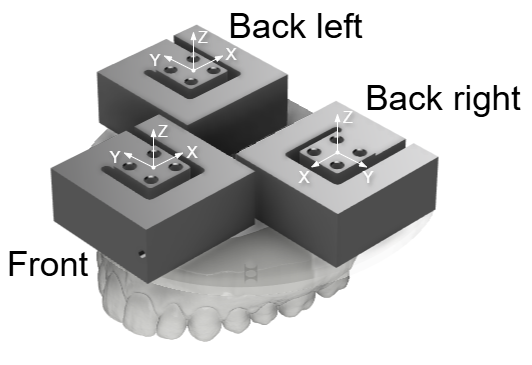
\includegraphics[width=\textwidth]{figures/load_cells_axis.drawio.png}
  \captionof{figure}{Load cells orientation.}
  \label{fig:load_cells_axis}
\end{minipage}

% \begin{figure}[H]
% \centering
% 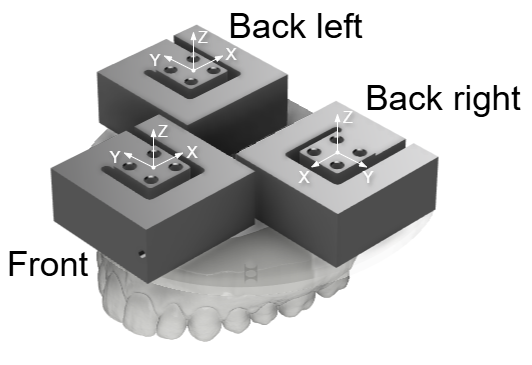
\includegraphics[width=0.4\textwidth]{figures/load_cells_axis.drawio.png}
% \caption{Load cells orientation.}
% \label{fig:load_cells_axis}
% \end{figure}

\subsection{Data acquisition and processing}
\label{sec:motion-capture}

\subsubsection{Subjects} 
Two healthy adult volunteers (author and project supervisor) participated in this pilot recording. Informed consent was obtained from both participants. 
Owing to time constraints and the exploratory nature of the study, no additional subjects were recruited. 

\subsubsection{Motion-capture acquisition}
\begin{minipage}{0.15\textwidth}
  \centering
  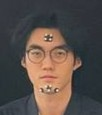
\includegraphics[width=\textwidth]{figures/benhui_marker.jpg}
  \captionof{figure}{Marker placement.}
  \label{fig:marker_placement}
\end{minipage}
\hfill
\begin{minipage}{0.80\textwidth}
Mandibular motion was recorded with a five-camera OptiTrack system sampling at 120 Hz.
Four reflective markers arranged in a square were attached to the forehead and served as a head-fixed reference frame.
A second set of three markers forming a triangle was placed on the gnathion. Figure~\ref{fig:marker_placement} shows the marker placement. 
Two additional lip markers were recorded but later discarded because a single marker cannot encode orientation \cite{motion_capture_adult,motion_capture_children}.
The subject then performed the motion sequences listed in Table~\ref{tab:recording-protocol}. Each frame was saved by Motive as a \texttt{.csv} file that contains
the 3-D marker positions (in millimetres) and the orientation of each marker set as quaternions. The calibrated volume had a residual error of $0.3\,$mm.
\end{minipage}

\begin{table}[H]
  \centering
  \small                                   
  \renewcommand{\arraystretch}{1.1}  
  \begin{tabularx}{\textwidth}{@{} c l l @{}}      
    \toprule
    \textbf{Food} & \textbf{Motion} & \textbf{\textit{Optional:} Duration} \\
    \midrule
    % ---------- Empty mouth block ----------
    Empty mouth & 20$\times$ open–close cycles                 & —     \\[1pt]
    \midrule
    % ---------- Chewing-gum block ----------
    \multirow{5}{*}{\parbox[c]{3.2cm}{\centering Chewing gum\\(Xylit-Pro,\\\emph{Excitemint})}}
      & Random side chewing                                    & 2 min \\[1pt]
      & Right-side chewing                                     & 1 min \\[1pt]
      & Left-side chewing                                      & 1 min \\[1pt]
      & Front-teeth-only chewing                               & 1 min \\ 
    \midrule
    % ---------- Biscuit block ----------
    \multirow{5}{*}{\parbox[c]{3.2cm}{\centering Biscuits\\(Bretzeli, \emph{Kambli})}}
      & random chewing                                    & — \\[1pt]
      & front-teeth chew → right-side chew                & — \\[1pt]
      & front-teeth chew → left-side chew                  & — \\[1pt]
      & \textit{fast} random chewing                      & — \\[1pt]
      & \textit{slow} random chewing                       & — \\
    \bottomrule
  \end{tabularx}
  \caption{Recording protocol. \textit{Notes:}  
  For chewing-gum trials the first run began with an unchewed piece and the same gum was kept for all subsequent motions.  
  For biscuit trials each run started with an empty, closed mouth; the subject then placed a biscuit, chewed as instructed, and swallowed.}
  \label{tab:recording-protocol}
\end{table}

\subsubsection{Data processing}
To reduce high-frequency noise in the motion capture data, a 4th-order Butterworth low-pass filter was applied, with a cutoff frequency set at 6 Hz. This value 
was chosen based on reported human mastication frequencies, typically ranging from 1-3 Hz and up to 6 Hz when the subjects are instructed to chew at higher rates \cite{chewinf_frequencies_2}.

Following filtering, the gnathion marker motion was transformed to the head-fixed marker reference frame using rotation matrices, effectively compensating 
for head motion during recording. The next step was to convert the data into the robot's coordinate system, defined as follows:
\begin{itemize}[nosep]
    \item the $X$ axis is horizontal, pointing to the subject's left;
    \item the $Y$ axis is horizontal, pointing forward;
    \item the $Z$ axis is vertical, pointing upwards.
\end{itemize}
Due to uncertainty about the absolute orientation of the OptiTrack coordinate system, we performed Principal Component Analysis (PCA) on the recorded open-close 
cycles to estimate the appropriate rotation matrix. The underlying assumption is that the largest motion range (i.e., the first principal component)
corresponds to the robot's Z-axis, the second to the Y-axis, and the third to the X-axis, following the hierarchy of motion amplitude typical in mastication 
dynamics during mouth opening \cite{mouth_opening_mvt}. As the principal components (PC) are orthogonal, the resulting matrix forms a valid orthonormal basis. The rotation matrix is 
then constructed by assigning the principal components as its column vectors.

Upon visual inspection of the data, we flipped the X and Z axes so that both decrease during jaw opening, ensuring alignment with the robot's coordinate 
conventions and human data \cite{chewing_traj}. All positional and rotational data were then projected into this new reference frame using the resulting rotation matrix:
\[
R = \begin{pmatrix}
    -\text{PC}_1 & \text{PC}_2 & -\text{PC}_3
\end{pmatrix}.
\]

To express orientation, the recorded quaternions were converted to Euler angles, providing the roll, pitch, and yaw components used by the robot's 
Stewart platform.

Then, to align the trajectory with the robot's origin, positional and rotational offsets were computed from the final stationary segment of the 
recording. The last second of the dataset—during which the subject remained still—was used to compute the median values of position and orientation. 
These offsets were subtracted from the full dataset to ensure proper alignment with the robot's neutral pose.

Finally, the most suitable trajectory segments were selected for replay on the robot. Selection was based on the 
smoothness of motion and the absence of outliers or artifacts in the recorded data.






